\documentclass{beamer}

\usepackage{graphicx}
\usepackage{epstopdf}
\usepackage{animate}
\graphicspath{{../fig/}}

\usepackage{amsmath}
\usepackage{amssymb}
\usepackage{amsfonts}
\usepackage{amsthm}
\usepackage{mathtools}
\usepackage{bm}
\usepackage{esvect}
\mathtoolsset{showonlyrefs}
\usefonttheme[onlymath]{serif}

\DeclareMathOperator{\trace}{tr}
\DeclareMathOperator{\rank}{\rho}
\newcommand*{\Round}[1]{\left(#1\right)}
\newcommand*{\Curly}[1]{\left\{#1\right\}}
\newcommand*{\Set}[1]{\Curly{#1}}
\newcommand*{\Prod}{\,}
\newcommand*{\Bold}[1]{\boldsymbol{\mathbf{#1}}}
\newcommand*{\Matr}[1]{\Bold{#1}}
\newcommand*{\Vect}[1]{\vv{\Bold{#1}}}
\newcommand*{\Inv}[1]{{#1}^{-1}}
\newcommand*{\Transp}[1]{{#1}^{T}}
\newcommand*{\Trace}[1]{\trace\Round{#1}}
\newcommand*{\Rank}[1]{\rank\Round{#1}}
\newcommand*{\ForAll}{\:\:\forall\,}
\newcommand*{\Viff}{\\\Updownarrow\\}
\newcommand*{\Vimplies}{\\\Downarrow\\}

\usepackage{siunitx}
\sisetup{output-decimal-marker = {,}}
\sisetup{exponent-product = {\cdot}}

\usepackage{pgffor}

\addtobeamertemplate{navigation symbols}{}{
  \usebeamerfont{footline}
  \usebeamercolor[fg]{footline}
  \hspace{1em}
  \raisebox{1.4pt}[0pt][0pt]{\insertframenumber/\inserttotalframenumber}
}

\makeatletter
\g@addto@macro\normalsize{
\setlength\abovedisplayskip{5pt}
\setlength\belowdisplayskip{5pt}
\setlength\abovedisplayshortskip{5pt}
\setlength\belowdisplayshortskip{5pt}
}
\makeatother

\renewcommand{\Prod}{\,}

\title{Estimativa da Região de Atração de Sistema Não-Linear em formato DAR por LMIs}
\author{Guilherme de Paoli Beal}
\institute{
  Universidade Federal do Rio Grande do Sul
  \\
  Programa de Pós-Graduação em Engenharia Elétrica
  \\
  ELE312 -- Sistemas Não-Lineares
}
\date{Junho de 2023}

\begin{document}

{
\setbeamertemplate{navigation symbols}{}
\begin{frame}[noframenumbering,label={frame:title}]
  \titlepage
\end{frame}
}

\begin{frame}\frametitle{Definição do Problema}
  \begin{itemize}
    \item Sistema não-linear, autônomo e não-forçado
    \begin{equation}
      \dot{\Vect{x}} = \Vect{f}\Round{\Vect{x}}
    \end{equation}
      \item A origem é um ponto de equilíbrio estável
    \begin{equation}
      \Vect{f}\Round{\Vect{0}} = \Vect{0}
    \end{equation}
      \item \emph{Região de Atração da Origem}
    \begin{equation}
      \Vect{x}(t_0) \in \mathcal{R}
      \implies
      \lim_{t \to \infty} \Vect{x}(t) = \Vect{0}
    \end{equation}
    \item $\Vect{x} \in \mathcal{B}_x$ -- Estados
    \item $\mathcal{B}_x \subset \mathbb{R}^n$ -- Região politópica
    \item $\Vect{f} \colon \mathbb{R}^n \to \mathbb{R}^n$ -- Função dinâmica localmente Lipschitz
    \item $\mathcal{R} \subset \mathcal{B}_x$ -- Região de Atração da Origem
  \end{itemize}
\end{frame}

\begin{frame}\frametitle{Representação Diferencial Algébrica (DAR)}
  \begin{itemize}
    \item Vetor auxiliar contendo termos polinômiais e racionais em $\Vect{x}$
    \item Matrizes afins em $\Vect{x}$
    \begin{gather}
      \left\{\begin{aligned}
        \dot{\Vect{x}} &= \Matr{A}_1\Round{\Vect{x}} \Prod \Vect{x} + \Matr{A}_2\Round{\Vect{x}} \Prod \Vect{z}\Round{\Vect{x}}
        \\
        \Vect{0} &= \Matr{\Omega}_1\Round{\Vect{x}} \Prod \Vect{x} + \Matr{\Omega}_2\Round{\Vect{x}} \Prod \Vect{z}\Round{\Vect{x}}
      \end{aligned}\right.
      \\
      \Rank{\Matr{\Omega}_2\Round{\Vect{x}}} = n_z \ForAll \Vect{x} \in \mathcal{B}_x
      \\
      \Vect{z}\Round{\Vect{x}} = -\Inv{\Matr{\Omega}_2\Round{\Vect{x}}} \Prod \Matr{\Omega}_1\Round{\Vect{x}} \Prod \Vect{x}
    \end{gather}
    \item $\Vect{z} \colon \mathbb{R}^n \to \mathbb{R}^{n_z}$
    \item $\Matr{A}_1 \colon \mathbb{R}^n \to \mathbb{R}^{n \times n}$
    \item $\Matr{A}_2 \colon \mathbb{R}^n \to \mathbb{R}^{n \times n_z}$
    \item $\Matr{\Omega}_1 \colon \mathbb{R}^n \to \mathbb{R}^{n_z \times n}$
    \item $\Matr{\Omega}_2 \colon \mathbb{R}^n \to \mathbb{R}^{n_z \times n_z}$
  \end{itemize}
\end{frame}

\begin{frame}<1>[label={frame:example1}]\frametitle<1>{Representação Diferencial Algébrica (DAR)}\frametitle<2>{Exemplos}\framesubtitle{Exemplo 1}
  \vspace{-20pt}
  \begin{equation}
    \left\{\begin{aligned}
      \dot{\Vect{x}} &= \Matr{A}_1\Round{\Vect{x}} \Prod \Vect{x} + \Matr{A}_2\Round{\Vect{x}} \Prod \Vect{z}\Round{\Vect{x}}
      \\
      \Vect{0} &= \Matr{\Omega}_1\Round{\Vect{x}} \Prod \Vect{x} + \Matr{\Omega}_2\Round{\Vect{x}} \Prod \Vect{z}\Round{\Vect{x}}
    \end{aligned}\right.
  \end{equation}
  \begin{align}
    \Vect{f}\Round{\Vect{x}}
    &= \begin{bmatrix}
      x_2
      \\
      -x_1 -x_2 + \frac{1}{3} \Prod {x_1}^3
    \end{bmatrix}
    &
    \Vect{x}
    &= \begin{bmatrix} x_1 \\ x_2 \end{bmatrix}
    &
    n &= 2
  \end{align}
  \begin{itemize}
    \item Vetor auxiliar polinomial em $\Vect{x}$
    \begin{align}
      \Vect{z}\Round{\Vect{x}} &= \begin{bmatrix} {x_1}^2 \end{bmatrix}
      &
      n_z &= 1
    \end{align}
    \item Matrizes afins em $\Vect{x}$
    \begin{align}
      \Matr{A}_1\Round{\Vect{x}}
      &= \begin{bmatrix}
         0 &  1 \\
        -1 & -1 \\
      \end{bmatrix}
      &
      \Matr{A}_2\Round{\Vect{x}}
      &= \begin{bmatrix}
        0                     \\
        \frac{1}{3} \Prod x_1 \\
      \end{bmatrix}
      \\
      \Matr{\Omega}_1\Round{\Vect{x}}
      &= \begin{bmatrix}
        x_1 & 0 \\
      \end{bmatrix}
      &
      \Matr{\Omega}_2\Round{\Vect{x}}
      &= \begin{bmatrix}
        -1 \\
      \end{bmatrix}
    \end{align}
  \end{itemize}
\end{frame}

\begin{frame}\frametitle{Representação Diferencial Algébrica (DAR)}\framesubtitle{Exemplo 1}
  \vspace{-20pt}
  \begin{equation}
    \left\{\begin{aligned}
      \dot{\Vect{x}} &= \Matr{A}_1\Round{\Vect{x}} \Prod \Vect{x} + \Matr{A}_2\Round{\Vect{x}} \Prod \Vect{z}\Round{\Vect{x}}
      \\
      \Vect{0} &= \Matr{\Omega}_1\Round{\Vect{x}} \Prod \Vect{x} + \Matr{\Omega}_2\Round{\Vect{x}} \Prod \Vect{z}\Round{\Vect{x}}
    \end{aligned}\right.
  \end{equation}
  \begin{align}
    \Vect{f}\Round{\Vect{x}}
    &= \begin{bmatrix}
      x_2
      \\
      -x_1 -x_2 + \frac{1}{3} \Prod {x_1}^3
    \end{bmatrix}
    &
    \Vect{x}
    &= \begin{bmatrix} x_1 \\ x_2 \end{bmatrix}
    &
    n &= 2
  \end{align}
  \begin{itemize}
    \item Vetor auxiliar polinomial em $\Vect{x}$
    \begin{align}
      \Vect{z}\Round{\Vect{x}} &= \begin{bmatrix} {x_1}^2 \\ {x_1}^3 \end{bmatrix}
      &
      n_z &= 2
    \end{align}
    \item Matrizes afins em $\Vect{x}$
    \begin{align}
      \Matr{A}_1\Round{\Vect{x}}
      &= \begin{bmatrix}
         0 &  1 \\
        -1 & -1 \\
      \end{bmatrix}
      &
      \Matr{A}_2\Round{\Vect{x}}
      &= \begin{bmatrix}
        0 & 0           \\
        0 & \frac{1}{3} \\
      \end{bmatrix}
      \\
      \Matr{\Omega}_1\Round{\Vect{x}}
      &= \begin{bmatrix}
        x_1 & 0 \\
        0   & 0 \\
      \end{bmatrix}
      &
      \Matr{\Omega}_2\Round{\Vect{x}}
      &= \begin{bmatrix}
        -1  & 0  \\
        x_1 & -1 \\
      \end{bmatrix}
    \end{align}
  \end{itemize}
\end{frame}

\begin{frame}<1>[label={frame:example2}]\frametitle<1>{Representação Diferencial Algébrica (DAR)}\frametitle<2>{Exemplos}\framesubtitle{Exemplo 2}
  \vspace{-20pt}
  \begin{equation}
    \left\{\begin{aligned}
      \dot{\Vect{x}} &= \Matr{A}_1\Round{\Vect{x}} \Prod \Vect{x} + \Matr{A}_2\Round{\Vect{x}} \Prod \Vect{z}\Round{\Vect{x}}
      \\
      \Vect{0} &= \Matr{\Omega}_1\Round{\Vect{x}} \Prod \Vect{x} + \Matr{\Omega}_2\Round{\Vect{x}} \Prod \Vect{z}\Round{\Vect{x}}
    \end{aligned}\right.
  \end{equation}
  \begin{align}
    \Vect{f}\Round{\Vect{x}}
    &= \begin{bmatrix}
      -x_2
      \\
      x_1 -x_2 -{x_1}^2 \Prod x_2 + \num{0.1} \Prod {x_1}^4 \Prod x_2
    \end{bmatrix}
    &
    \Vect{x}
    &= \begin{bmatrix} x_1 \\ x_2 \end{bmatrix}
    &
    n &= 2
  \end{align}
  \begin{itemize}
    \item Vetor auxiliar polinomial em $\Vect{x}$
    \begin{align}
      \Transp{\Vect{z}\Round{\Vect{x}}} &= \begin{bmatrix} {x_1}^2 & {x_1}^3 & {x_1}^4 \end{bmatrix}
      &
      n_z &= 3
    \end{align}
    \item Matrizes afins em $\Vect{x}$
    \begin{align}
      \Matr{A}_1\Round{\Vect{x}}
      &= \begin{bmatrix}
        0 & -1 \\
        1 & -1 \\
      \end{bmatrix}
      &
      \Matr{A}_2\Round{\Vect{x}}
      &= \begin{bmatrix}
        0    & 0 & 0                   \\
        -x_2 & 0 & \num{0.1} \Prod x_2 \\
      \end{bmatrix}
      \\
      \Matr{\Omega}_1\Round{\Vect{x}}
      &= \begin{bmatrix}
        x_1 & 0 \\
        0   & 0 \\
        0   & 0 \\
      \end{bmatrix}
      &
      \Matr{\Omega}_2\Round{\Vect{x}}
      &= \begin{bmatrix}
        -1  & 0   & 0  \\
        x_1 & -1  & 0  \\
        0   & x_1 & -1 \\
      \end{bmatrix}
    \end{align}
  \end{itemize}
\end{frame}

\begin{frame}\frametitle{Função de Lyapunov}
  \begin{itemize}
    \item Função positiva definida
    % \begin{equation}
    %   \varepsilon_1 \Prod \Transp{\Vect{x}} \Prod \Vect{x} \leq V\Round{\Vect{x}} \leq \varepsilon_2 \Prod \Transp{\Vect{x}} \Prod \Vect{x}
    %   \ForAll \Vect{x} \in \mathcal{B}_x
    % \end{equation}
    \begin{gather}
      V\Round{\Vect{x}} > 0 \ForAll \Vect{x} \in \mathcal{B}_x \setminus \Set{\Vect{0}}
      \\
      V\Round{\Vect{0}} = 0
    \end{gather}
    \item Derivada da função negativa definida
    % \begin{equation}
    %   \dot{V}\Round{\Vect{x}} \leq -\varepsilon_3 \Prod \Transp{\Vect{x}} \Prod \Vect{x}
    %   \ForAll \Vect{x} \in \mathcal{B}_x
    % \end{equation}
    \begin{gather}
      \dot{V}\Round{\Vect{x}} < 0 \ForAll \Vect{x} \in \mathcal{B}_x \setminus \Set{\Vect{0}}
      \\
      \dot{V}\Round{\Vect{0}} = 0
    \end{gather}
    \item Estimativa da região de atração da origem
    \begin{equation}
      \hat{\mathcal{R}} = \left\{\Vect{x} \in \mathcal{B}_x \colon V\Round{\Vect{x}} \leq 1\right\}
    \end{equation}
    \item $V \colon \mathcal{B}_x \to \mathbb{R}$ -- Função de Lyapunov
    % \item $\varepsilon_1 \in \mathbb{R}^+$ -- Constante Positiva
    % \item $\varepsilon_2 \in \mathbb{R}^+$ -- Constante Positiva
    % \item $\varepsilon_3 \in \mathbb{R}^+$ -- Constante Positiva
    \item $\hat{\mathcal{R}} \subset \mathcal{R}$ -- Estimativa da região de Atração da Origem
  \end{itemize}
\end{frame}

\begin{frame}\frametitle{Função de Lyapunov}\framesubtitle{Função Quadrática}
  \begin{gather}
    V\Round{\Vect{x}}= \Transp{\Vect{x}} \Prod \Matr{P} \Prod \Vect{x}
    \\
    \Matr{P} = \Transp{\Matr{P}} \succ 0
    \\
    \begin{aligned}
      \dot{V}\Round{\Vect{x}}
      &= \Transp{\dot{\Vect{x}}} \Prod \Matr{P} \Prod \Vect{x} + \Transp{\Vect{x}} \Prod \Matr{P} \Prod \dot{\Vect{x}}
      \\
      &= \Transp{\Vect{f}\Round{\Vect{x}}} \Prod \Matr{P} \Prod \Vect{x} + \Transp{\Vect{x}} \Prod \Matr{P} \Prod \Vect{f}\Round{\Vect{x}}
    \end{aligned}
  \end{gather}
  \begin{itemize}
    \item $\Matr{P} \in \mathbb{R}^{n \times n}$
  \end{itemize}
\end{frame}

\begin{frame}\frametitle{Função de Lyapunov}\framesubtitle{Função Quadrática -- Representação Estendida}
  \begin{itemize}
    \item Vetor estendido
    \begin{gather}
      \begin{aligned}
        \Vect{\zeta}\Round{\Vect{x}}
        &= \begin{bmatrix} \Vect{x} \\ \dot{\Vect{x}} \\ \Vect{z}\Round{\Vect{x}} \end{bmatrix}
        &
        \Matr{\mathcal{M}}\Round{\Vect{x}}
        &= \begin{bmatrix}
          \Matr{A}_1\Round{\Vect{x}}      & -\Matr{I}_n & \Matr{A}_2\Round{\Vect{x}}      \\
          \Matr{\Omega}_1\Round{\Vect{x}} & \Matr{0}    & \Matr{\Omega}_2\Round{\Vect{x}} \\
        \end{bmatrix}
      \end{aligned}
      \\
      \Matr{\mathcal{M}}\Round{\Vect{x}} \Prod \Vect{\zeta}\Round{\Vect{x}} = \vec{0}
    \end{gather}
    \item Função de Lyapunov
    \small
    \begin{align}
      V\Round{\Vect{x}}
      &= \Transp{\Vect{\zeta}\Round{\Vect{x}}} \Prod \Matr{\Sigma}(\Matr{P}) \Prod \Vect{\zeta}\Round{\Vect{x}} \geq 0
      &
      \dot{V}\Round{\Vect{x}}
      &= \Transp{\Vect{\zeta}\Round{\Vect{x}}} \Prod \Matr{\Lambda}(\Matr{P}) \Prod \Vect{\zeta}\Round{\Vect{x}} \leq 0
    \end{align}
    \normalsize
    \vspace{-18pt}
    \begin{align}
    \Matr{\Sigma}(\Matr{P})
      &= \begin{bmatrix}
        \Matr{P}  & \Matr{0}   & \Matr{0}       \\
        \Matr{0}  & \Matr{0}_n & \Matr{0}       \\
        \Matr{0}  & \Matr{0}   & \Matr{0}_{n_z} \\
      \end{bmatrix}
      &
      \Matr{\Lambda}(\Matr{P})
      &= \begin{bmatrix}
        \Matr{0}_n & \Matr{P}   & \Matr{0}       \\
        \Matr{P}   & \Matr{0}_n & \Matr{0}       \\
        \Matr{0}   & \Matr{0}   & \Matr{0}_{n_z} \\
      \end{bmatrix}
    \end{align}
    \item $\Vect{\zeta} \colon \mathbb{R}^n \to \mathbb{R}^{2 \Prod n + n_z}$
    \item $\Matr{\mathcal{M}} \colon \mathbb{R}^n \to \mathbb{R}^{(n + n_z) \times (2 \Prod n + n_z)}$
    \item $\Matr{\Sigma} \colon \mathbb{R}^{n \times n} \to \mathbb{R}^{(2 \Prod n + n_z) \times (2 \Prod n + n_z)}$
    \item $\Matr{\Lambda} \colon \mathbb{R}^{n \times n} \to \mathbb{R}^{(2 \Prod n + n_z) \times (2 \Prod n + n_z)}$
  \end{itemize}
\end{frame}

\begin{frame}\frametitle{Politopo}
  \begin{itemize}
    \item Região delimitada por suas $n_e$ faces $\Vect{h}_k$
    \begin{equation}
      \mathcal{B}_x
      = \Set{\Vect{x} \in \mathbb{R}^n \colon \Transp{\Vect{h}_k} \Prod \Vect{x} \leq 1 \,,\; k = 1, \dotsc, n_e}
    \end{equation}
    \item Ajustando para o vetor estendido
    \begin{gather}
      \mathcal{B}_x
      = \Set{\Vect{x} \in \mathbb{R}^n \colon \Transp{\Vect{\vartheta}\Round{\Vect{h}_k}} \Prod \Vect{\zeta}\Round{\Vect{x}} \leq 1 \,,\; k = 1, \dotsc, n_e}
      \\
      \Vect{\vartheta}\Round{\Vect{h}_k} = \begin{bmatrix} \Vect{h}_k \\ \Vect{0}_n \\ \Vect{0}_{n_z} \end{bmatrix}
    \end{gather}
    \item $\Vect{h}_k \in \mathbb{R}^n$
    \item $n_e \in \mathbb{N}$
    \item $\Vect{\vartheta} \colon \mathbb{R}^n \to \mathbb{R}^{2 \Prod n + n_z}$
  \end{itemize}
\end{frame}

\begin{frame}\frametitle{Estimativa da Região de Atração da Origem}
  \begin{itemize}
    \item O interior de uma curva de nível da função de Lyapunov no interior do politopo é uma estimativa da região de atração da origem
    \begin{gather}
      \hat{\mathcal{R}} \subset \mathcal{B}_x
      \Viff
      \Transp{\Vect{h}_k} \Prod \Vect{x} \leq 1
      \ForAll \Vect{x} \colon V\Round{\Vect{x}} \leq 1
      % \,,\; k = 1, \dotsc, n_e
      \Viff
      \Transp{\Vect{\vartheta}\Round{\Vect{h}_k}} \Prod \Vect{\zeta}\Round{\Vect{x}} \leq 1
      \ForAll \Vect{x} \in \mathbb{R}^n \colon \Transp{\Vect{\zeta}\Round{\Vect{x}}} \Prod \Matr{\Sigma}(\Matr{P}) \Prod \Vect{\zeta}\Round{\Vect{x}} \leq 1
      % \,,\\ k = 1, \dotsc, n_e
      \Viff
      2 \Prod \Transp{\Vect{\vartheta}\Round{\Vect{h}_k}} \Prod \Vect{\zeta}\Round{\Vect{x}} - 2 \leq 0
      \ForAll \Vect{x} \colon \Transp{\Vect{\zeta}\Round{\Vect{x}}} \Prod \Matr{\Sigma}(\Matr{P}) \Prod \Vect{\zeta}\Round{\Vect{x}} -1 \leq 0
      % \,,\\ k = 1, \dotsc, n_e
      \\ k = 1, \dotsc, n_e
    \end{gather}
  \end{itemize}
\end{frame}

\begin{frame}\frametitle{Estimativa da Região de Atração da Origem}
  \begin{itemize}
    \item \textit{S-Procedure}
    \small
    \begin{gather}
      \Transp{\Vect{v}} \Prod \Matr{T}_1 \Prod \Vect{v} + 2 \Prod \Transp{\Vect{u}_1} \Prod \Vect{v} + w_1 \leq 0
      \implies
      \Transp{\Vect{v}} \Prod \Matr{T}_2 \Prod \Vect{v} + 2 \Prod \Transp{\Vect{u}_2} \Prod \Vect{v} + w_2 \leq 0
      \Viff
      \Transp{\begin{bmatrix} \Vect{v} \\ 1 \end{bmatrix}} \Round{\begin{bmatrix} \Matr{T}_1 & \Vect{u}_1 \\ \Transp{\Vect{u}_1} & w_1 \end{bmatrix} - \lambda \begin{bmatrix} \Matr{T}_2 & \Vect{u}_2 \\ \Transp{\Vect{u}_2} & w_2 \end{bmatrix}} \begin{bmatrix} \Vect{v} \\ 1 \end{bmatrix} \geq 0
      ,\; \lambda \geq 0
    \end{gather}
    \normalsize
    \item Curva de nível no interior do politopo
    \small
    \begin{gather}
      \Transp{\Vect{\zeta}\Round{\Vect{x}}} \Prod \Matr{\Sigma}(\Matr{P}) \Prod \Vect{\zeta}\Round{\Vect{x}} -1 \leq 0
      \implies
      2 \Prod \Transp{\Vect{\vartheta}\Round{\Vect{h}_k}} \Prod \Vect{\zeta}\Round{\Vect{x}} - 2 \leq 0
      \Viff
      \Transp{\begin{bmatrix} \Vect{\zeta}\Round{\Vect{x}} \\ 1 \end{bmatrix}} \Round{\begin{bmatrix} \Matr{\Sigma}(\Matr{P}) & \Vect{0} \\ \Transp{\Vect{0}} & -1 \end{bmatrix} - \nu \begin{bmatrix} \Matr{0} & \Vect{\vartheta}\Round{\Vect{h}_k} \\ \Transp{\Vect{\vartheta}\Round{\Vect{h}_k}} & -2 \end{bmatrix}} \begin{bmatrix} \Vect{\zeta}\Round{\Vect{x}} \\ 1 \end{bmatrix} \geq 0
      ,\\ \nu \geq 0
      % ,\\ k = 1, \dotsc, n_e
    \end{gather}
    \normalsize
  \end{itemize}
\end{frame}

\begin{frame}\frametitle{Estimativa da Região de Atração da Origem}
  \begin{itemize}
    \item Vetor estendido
    \begin{gather}
      \begin{aligned}
        \Vect{\varsigma}\Round{\Vect{x}}
        &= \begin{bmatrix} \Vect{\zeta}\Round{\Vect{x}} \\ 1 \end{bmatrix}
        &
        \Matr{\mathcal{N}}\Round{\Vect{x}}
        &= \begin{bmatrix}
          \Matr{A}_1\Round{\Vect{x}}      & -\Matr{I}_n & \Matr{A}_2\Round{\Vect{x}}      & \Vect{0} \\
          \Matr{\Omega}_1\Round{\Vect{x}} & \Matr{0}    & \Matr{\Omega}_2\Round{\Vect{x}} & \Vect{0} \\
          -\Matr{I}_n                     & \Matr{0}    & \Matr{0}                        & \Vect{x} \\
        \end{bmatrix}
      \end{aligned}
      \\
      \Matr{\mathcal{N}}\Round{\Vect{x}} \Prod \Vect{\varsigma}\Round{\Vect{x}} = \Vect{0}
    \end{gather}
    \item Curva de nível no iterior do politopo
    \begin{gather}
      \Transp{\Vect{\varsigma}\Round{\Vect{x}}} \Prod \Matr{\Pi}(\Matr{P}, \Vect{h}_k, \nu) \Prod \Vect{\varsigma}\Round{\Vect{x}} \geq 0
      \,,\; k = 1, \dotsc, n_e
      \\
      \Matr{\Pi}(\Matr{P}, \Vect{h}_k, \nu) = \begin{bmatrix}
        \Matr{\Sigma}(\Matr{P})                          & -\nu \Prod \Vect{\vartheta}(\Vect{h}_k) \\
        -\nu \Prod \Transp{\Vect{\vartheta}(\Vect{h}_k)} & 2 \Prod \nu - 1                         \\
      \end{bmatrix}
    \end{gather}
    \item $\Vect{\varsigma} \colon \mathbb{R}^n \to \mathbb{R}^{2 \Prod n + n_z + 1}$
    \item $\Matr{\Pi} \colon \mathbb{R}^{n \times n} \times \mathbb{R}^n \times \mathbb{R} \to \mathbb{R}^{(2 \Prod n + n_z + 1) \times (2 \Prod n + n_z + 1)}$
    \item $\Matr{\mathcal{N}} \colon \mathbb{R}^n \to \mathbb{R}^{(2 \Prod n + n_z) \times (2 \Prod n + n_z + 1)}$
    \item $\nu \in \mathbb{R}^+$
  \end{itemize}
\end{frame}

\begin{frame}\frametitle{Inequações Matriciais Lineares (LMIs)}
  \begin{itemize}
    \item Lema de Finsler
    \begin{gather}
      \left\{\begin{aligned}
        &\Transp{\Vect{v}(\Vect{x})} \Prod \Matr{T}(\Vect{x}) \Prod \Vect{v}(\Vect{x}) > 0
        \\
        &\Matr{\mathcal{O}}(\Vect{x}) \Prod \Vect{v}(\Vect{x}) = \Vect{0}
      \end{aligned}\right.
      \ForAll \Vect{x} \in \mathcal{B}_x
      \Vimplies
      \Matr{T}(\Vect{x}) + \Matr{K} \Prod \Matr{\mathcal{O}}(\Vect{x}) + \Transp{\Matr{\mathcal{O}}(\Vect{x})} \Prod \Transp{\Matr{K}} \succ 0
      \ForAll \Vect{x} \in \mathcal{V}(\mathcal{B}_x)
    \end{gather}
    \item Função de Lyapunov positiva definida
    \begin{gather}
      \left\{\begin{aligned}
        &\Transp{\Vect{\zeta}(\Vect{x})} \Prod \Matr{\Sigma}(\Matr{P}) \Prod \Vect{\zeta}(\Vect{x}) > 0
        \\
        &\Matr{\mathcal{M}}(\Vect{x}) \Prod \Vect{\zeta}(\Vect{x}) = \Vect{0}
      \end{aligned}\right.
      \ForAll \Vect{x} \in \mathcal{B}_x
      \Vimplies
      \Matr{\Sigma}(\Matr{P}) + \Matr{L} \Prod \Matr{\mathcal{M}}(\Vect{x}) + \Transp{\Matr{\mathcal{M}}(\Vect{x})} \Prod \Transp{\Matr{L}} \succ 0
      \ForAll \Vect{x} \in \mathcal{V}(\mathcal{B}_x)
    \end{gather}
    \item $\Matr{L} \in \mathbb{R}^{(2 \Prod n + n_z) \times (n + n_z)}$
  \end{itemize}
\end{frame}

\begin{frame}\frametitle{Inequações Matriciais Lineares (LMIs)}
  \begin{itemize}
    \item Lema de Finsler
    \begin{gather}
      \left\{\begin{aligned}
        &\Transp{\Vect{v}(\Vect{x})} \Prod \Matr{T}(\Vect{x}) \Prod \Vect{v}(\Vect{x}) > 0
        \\
        &\Matr{\mathcal{O}}(\Vect{x}) \Prod \Vect{v}(\Vect{x}) = \Vect{0}
      \end{aligned}\right.
      \ForAll \Vect{x} \in \mathcal{B}_x
      \Vimplies
      \Matr{T}(\Vect{x}) + \Matr{K} \Prod \Matr{\mathcal{O}}(\Vect{x}) + \Transp{\Matr{\mathcal{O}}(\Vect{x})} \Prod \Transp{\Matr{K}} \succ 0
      \ForAll \Vect{x} \in \mathcal{V}(\mathcal{B}_x)
    \end{gather}
    \item Derivada da função de Lyapunov negativa definida
    \begin{gather}
      \left\{\begin{aligned}
        &{-\Transp{\Vect{\zeta}(\Vect{x})}} \Prod \Matr{\Lambda}(\Matr{P}) \Prod \Vect{\zeta}(\Vect{x}) > 0
        \\
        &\Matr{\mathcal{M}}(\Vect{x}) \Prod \Vect{\zeta}(\Vect{x}) = \Vect{0}
      \end{aligned}\right.
      \ForAll \Vect{x} \in \mathcal{B}_x
      \Vimplies
      -\Matr{\Lambda}(\Matr{P}) + \Matr{W} \Prod \Matr{\mathcal{M}}(\Vect{x}) + \Transp{\Matr{\mathcal{M}}(\Vect{x})} \Prod \Transp{\Matr{W}} \succ 0
      \ForAll \Vect{x} \in \mathcal{V}(\mathcal{B}_x)
    \end{gather}
    \item $\Matr{W} \in \mathbb{R}^{(2 \Prod n + n_z) \times (n + n_z)}$
  \end{itemize}
\end{frame}

\begin{frame}\frametitle{Inequações Matriciais Lineares (LMIs)}
  \begin{itemize}
    \item Lema de Finsler
    \begin{gather}
      \left\{\begin{aligned}
        &\Transp{\Vect{v}(\Vect{x})} \Prod \Matr{T}(\Vect{x}) \Prod \Vect{v}(\Vect{x}) > 0
        \\
        &\Matr{\mathcal{O}}(\Vect{x}) \Prod \Vect{v}(\Vect{x}) = \Vect{0}
      \end{aligned}\right.
      \ForAll \Vect{x} \in \mathcal{B}_x
      \Vimplies
      \Matr{T}(\Vect{x}) + \Matr{K} \Prod \Matr{\mathcal{O}}(\Vect{x}) + \Transp{\Matr{\mathcal{O}}(\Vect{x})} \Prod \Transp{\Matr{K}} \succ 0
      \ForAll \Vect{x} \in \mathcal{V}(\mathcal{B}_x)
    \end{gather}
    \item Curva de nível da função de Lyapunov no interior do politopo
    \begin{gather}
      \left\{\begin{aligned}
        &\Transp{\Vect{\varsigma}(\Vect{x})} \Prod \Matr{\Pi}(\Matr{P}, \Vect{h}_k, \nu) \Prod \Vect{\varsigma}(\Vect{x}) > 0
        \\
        &\Matr{\mathcal{N}}(\Vect{x}) \Prod \Vect{\varsigma}(\Vect{x}) = \Vect{0}
      \end{aligned}\right.
      \ForAll \Vect{x} \in \mathcal{B}_x
      % ,\; k = 1, \dotsc, n_e
      \Vimplies
      \Matr{\Pi}(\Matr{P}, \Vect{h}_k, \nu) + \Matr{R}_k \Prod \Matr{\mathcal{N}}(\Vect{x}) + \Transp{\Matr{\mathcal{N}}(\Vect{x})} \Prod \Transp{\Matr{R}_k} \succ 0
      \ForAll \Vect{x} \in \mathcal{V}(\mathcal{B}_x)
      ,\\ k = 1, \dotsc, n_e
    \end{gather}
    \item $\Matr{R}_k \in \mathbb{R}^{(2 \Prod n + n_z + 1) \times (2 \Prod n + n_z)}$
  \end{itemize}
\end{frame}

\begin{frame}\frametitle{Inequações Matriciais Lineares (LMIs)}\framesubtitle{Otimização}
  \begin{itemize}
    \item A função de Lyapunov quadrática resulta em uma estimativa elipsoidal da região de atração da origem
    \item Maximização do tamanho dessa região
    \begin{itemize}
      \item maximização do menor eixo
      \item maximização do volume
      \item maximização em alguma direção
      \item minimização do traço
    \end{itemize}
    \begin{equation}
      \min_{\Matr{P}} \Trace{\Matr{P}}
    \end{equation}
  \end{itemize}
\end{frame}

\begin{frame}\frametitle{Inequações Matriciais Lineares (LMIs)}\framesubtitle{Resumo}
  \begin{gather}
    \min_{\Matr{P}} \Trace{\Matr{P}}
    \\
    \Matr{P} = \Transp{\Matr{P}} \succ 0
    \\
    \nu > 0
    \\
    \Matr{\Sigma}(\Matr{P}) + \Matr{L} \Prod \Matr{\mathcal{M}}(\Vect{x}) + \Transp{\Matr{\mathcal{M}}(\Vect{x})} \Prod \Transp{\Matr{L}} \succ 0
    \ForAll \Vect{x} \in \mathcal{V}(\mathcal{B}_x)
    \\
    -\Matr{\Lambda}(\Matr{P}) + \Matr{W} \Prod \Matr{\mathcal{M}}(\Vect{x}) + \Transp{\Matr{\mathcal{M}}(\Vect{x})} \Prod \Transp{\Matr{W}} \succ 0
    \ForAll \Vect{x} \in \mathcal{V}(\mathcal{B}_x)
    \\
    \Matr{\Pi}(\Matr{P}, \Vect{h}_k, \nu) + \Matr{R}_k \Prod \Matr{\mathcal{N}}(\Vect{x}) + \Transp{\Matr{\mathcal{N}}(\Vect{x})} \Prod \Transp{\Matr{R}_k} \succ 0
    \\\ForAll \Vect{x} \in \mathcal{V}(\mathcal{B}_x)
    ,\; k = 1, \dotsc, n_e
  \end{gather}
  \begin{itemize}
    \item O politopo é desconhecido
    \begin{itemize}
      \item Inicializa pequeno e aumenta enquanto o problema é factível
    \end{itemize}
  \end{itemize}
\end{frame}

\begin{frame}\frametitle{Exemplos}\framesubtitle{Politopo Losangular}
  \begin{equation}
    \mathcal{B}_x
    = \Set{\Vect{x} \in \mathbb{R}^n \colon \Transp{\Vect{h}_k} \Prod \Vect{x} \leq 1 \,,\; k = 1, \dotsc, n_e}
  \end{equation}
  \begin{itemize}
    \item Politopo losangular
    \begin{itemize}
      \item centrado na origem
      \item aresta de tamanho $a$
    \end{itemize}
    \begin{gather}
      n_e = 4
      \\
      \begin{aligned}
        \Vect{h}_1 &= \frac{1}{a} \Prod \begin{bmatrix} 1 \\ 1 \end{bmatrix}
        &
        \Vect{h}_2 &= \frac{1}{a} \Prod \begin{bmatrix} 1 \\ -1 \end{bmatrix}
        &
        \Vect{h}_3 &= \frac{1}{a} \Prod \begin{bmatrix} -1 \\ -1 \end{bmatrix}
        &
        \Vect{h}_4 &= \frac{1}{a} \Prod \begin{bmatrix} -1 \\ 1 \end{bmatrix}
      \end{aligned}
      \\
      \mathcal{V}(\mathcal{B}_x) = \left\{
      \begin{bmatrix} a \\ 0 \end{bmatrix}
      ,
      \begin{bmatrix} -a \\ 0 \end{bmatrix}
      ,
      \begin{bmatrix} 0 \\ a \end{bmatrix}
      ,
      \begin{bmatrix} 0 \\ -a \end{bmatrix}
      \right\}
    \end{gather}
    % \item Nos exemplos, $a_0 = \num{0.1}$, $a_i = a_{i-1} + \num{0.1}$
  \end{itemize}
\end{frame}

\begin{frame}\frametitle{Exemplos}\framesubtitle{Politopo Quadrado}
  \begin{equation}
    \mathcal{B}_x
    = \Set{\Vect{x} \in \mathbb{R}^n \colon \Transp{\Vect{h}_k} \Prod \Vect{x} \leq 1 \,,\; k = 1, \dotsc, n_e}
  \end{equation}
  \begin{itemize}
    \item Politopo quadrado
    \begin{itemize}
      \item centrado na origem
      \item aresta de tamanho $a$
    \end{itemize}
    \begin{gather}
      n_e = 4
      \\
      \begin{aligned}
        \Vect{h}_1 &= \frac{1}{a} \Prod \begin{bmatrix} 1 \\ 0 \end{bmatrix}
        &
        \Vect{h}_2 &= \frac{1}{a} \Prod \begin{bmatrix} 0 \\ -1 \end{bmatrix}
        &
        \Vect{h}_3 &= \frac{1}{a} \Prod \begin{bmatrix} -1 \\ 0 \end{bmatrix}
        &
        \Vect{h}_4 &= \frac{1}{a} \Prod \begin{bmatrix} 0 \\ 1 \end{bmatrix}
      \end{aligned}
      \\
      \mathcal{V}(\mathcal{B}_x) = \left\{
      \begin{bmatrix} a \\ a \end{bmatrix}
      ,
      \begin{bmatrix} a \\ -a \end{bmatrix}
      ,
      \begin{bmatrix} -a \\ -a \end{bmatrix}
      ,
      \begin{bmatrix} -a \\ a \end{bmatrix}
      \right\}
    \end{gather}
    % \item Nos exemplos, $a_0 = \num{0.1}$, $a_i = a_{i-1} + \num{0.1}$
  \end{itemize}
\end{frame}

\againframe<2>{frame:example1}

\begin{frame}\frametitle{Exemplos}\framesubtitle{Exemplo 1 - Politopo Losangular}
  \centering
  \animategraphics[loop,controls,width=0.85\linewidth]{6}{exemplo1_}{0}{28}
\end{frame}

\begin{frame}\frametitle{Exemplos}\framesubtitle{Exemplo 1 - Politopo Quadrado}
  \centering
  \animategraphics[loop,controls,width=0.85\linewidth]{6}{exemplo1_quadrado_}{0}{28}
\end{frame}

\begin{frame}\frametitle{Exemplos}\framesubtitle{Exemplo 1 - Politopo Losangular}
  \centering
  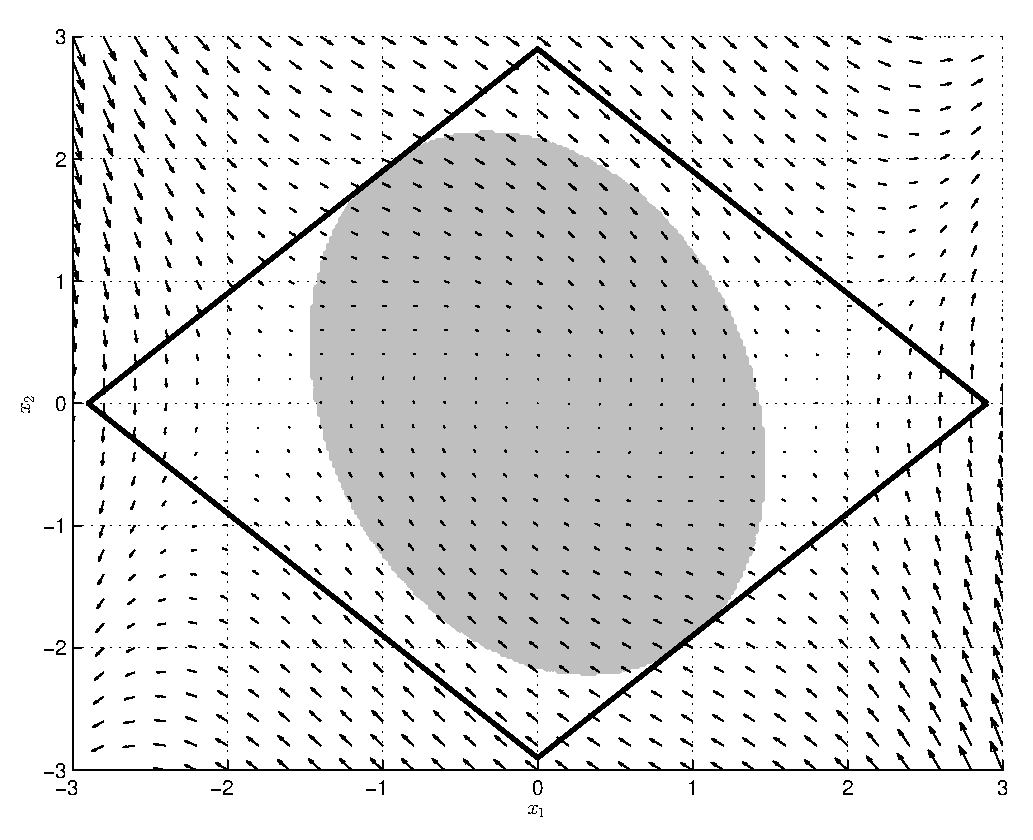
\includegraphics[height=0.7\textheight]{exemplo1_28.eps}
  \begin{equation}
    a = \num{2.9}
  \end{equation}
\end{frame}

\begin{frame}\frametitle{Exemplos}\framesubtitle{Exemplo 1 - Politopo Quadrado}
  \centering
  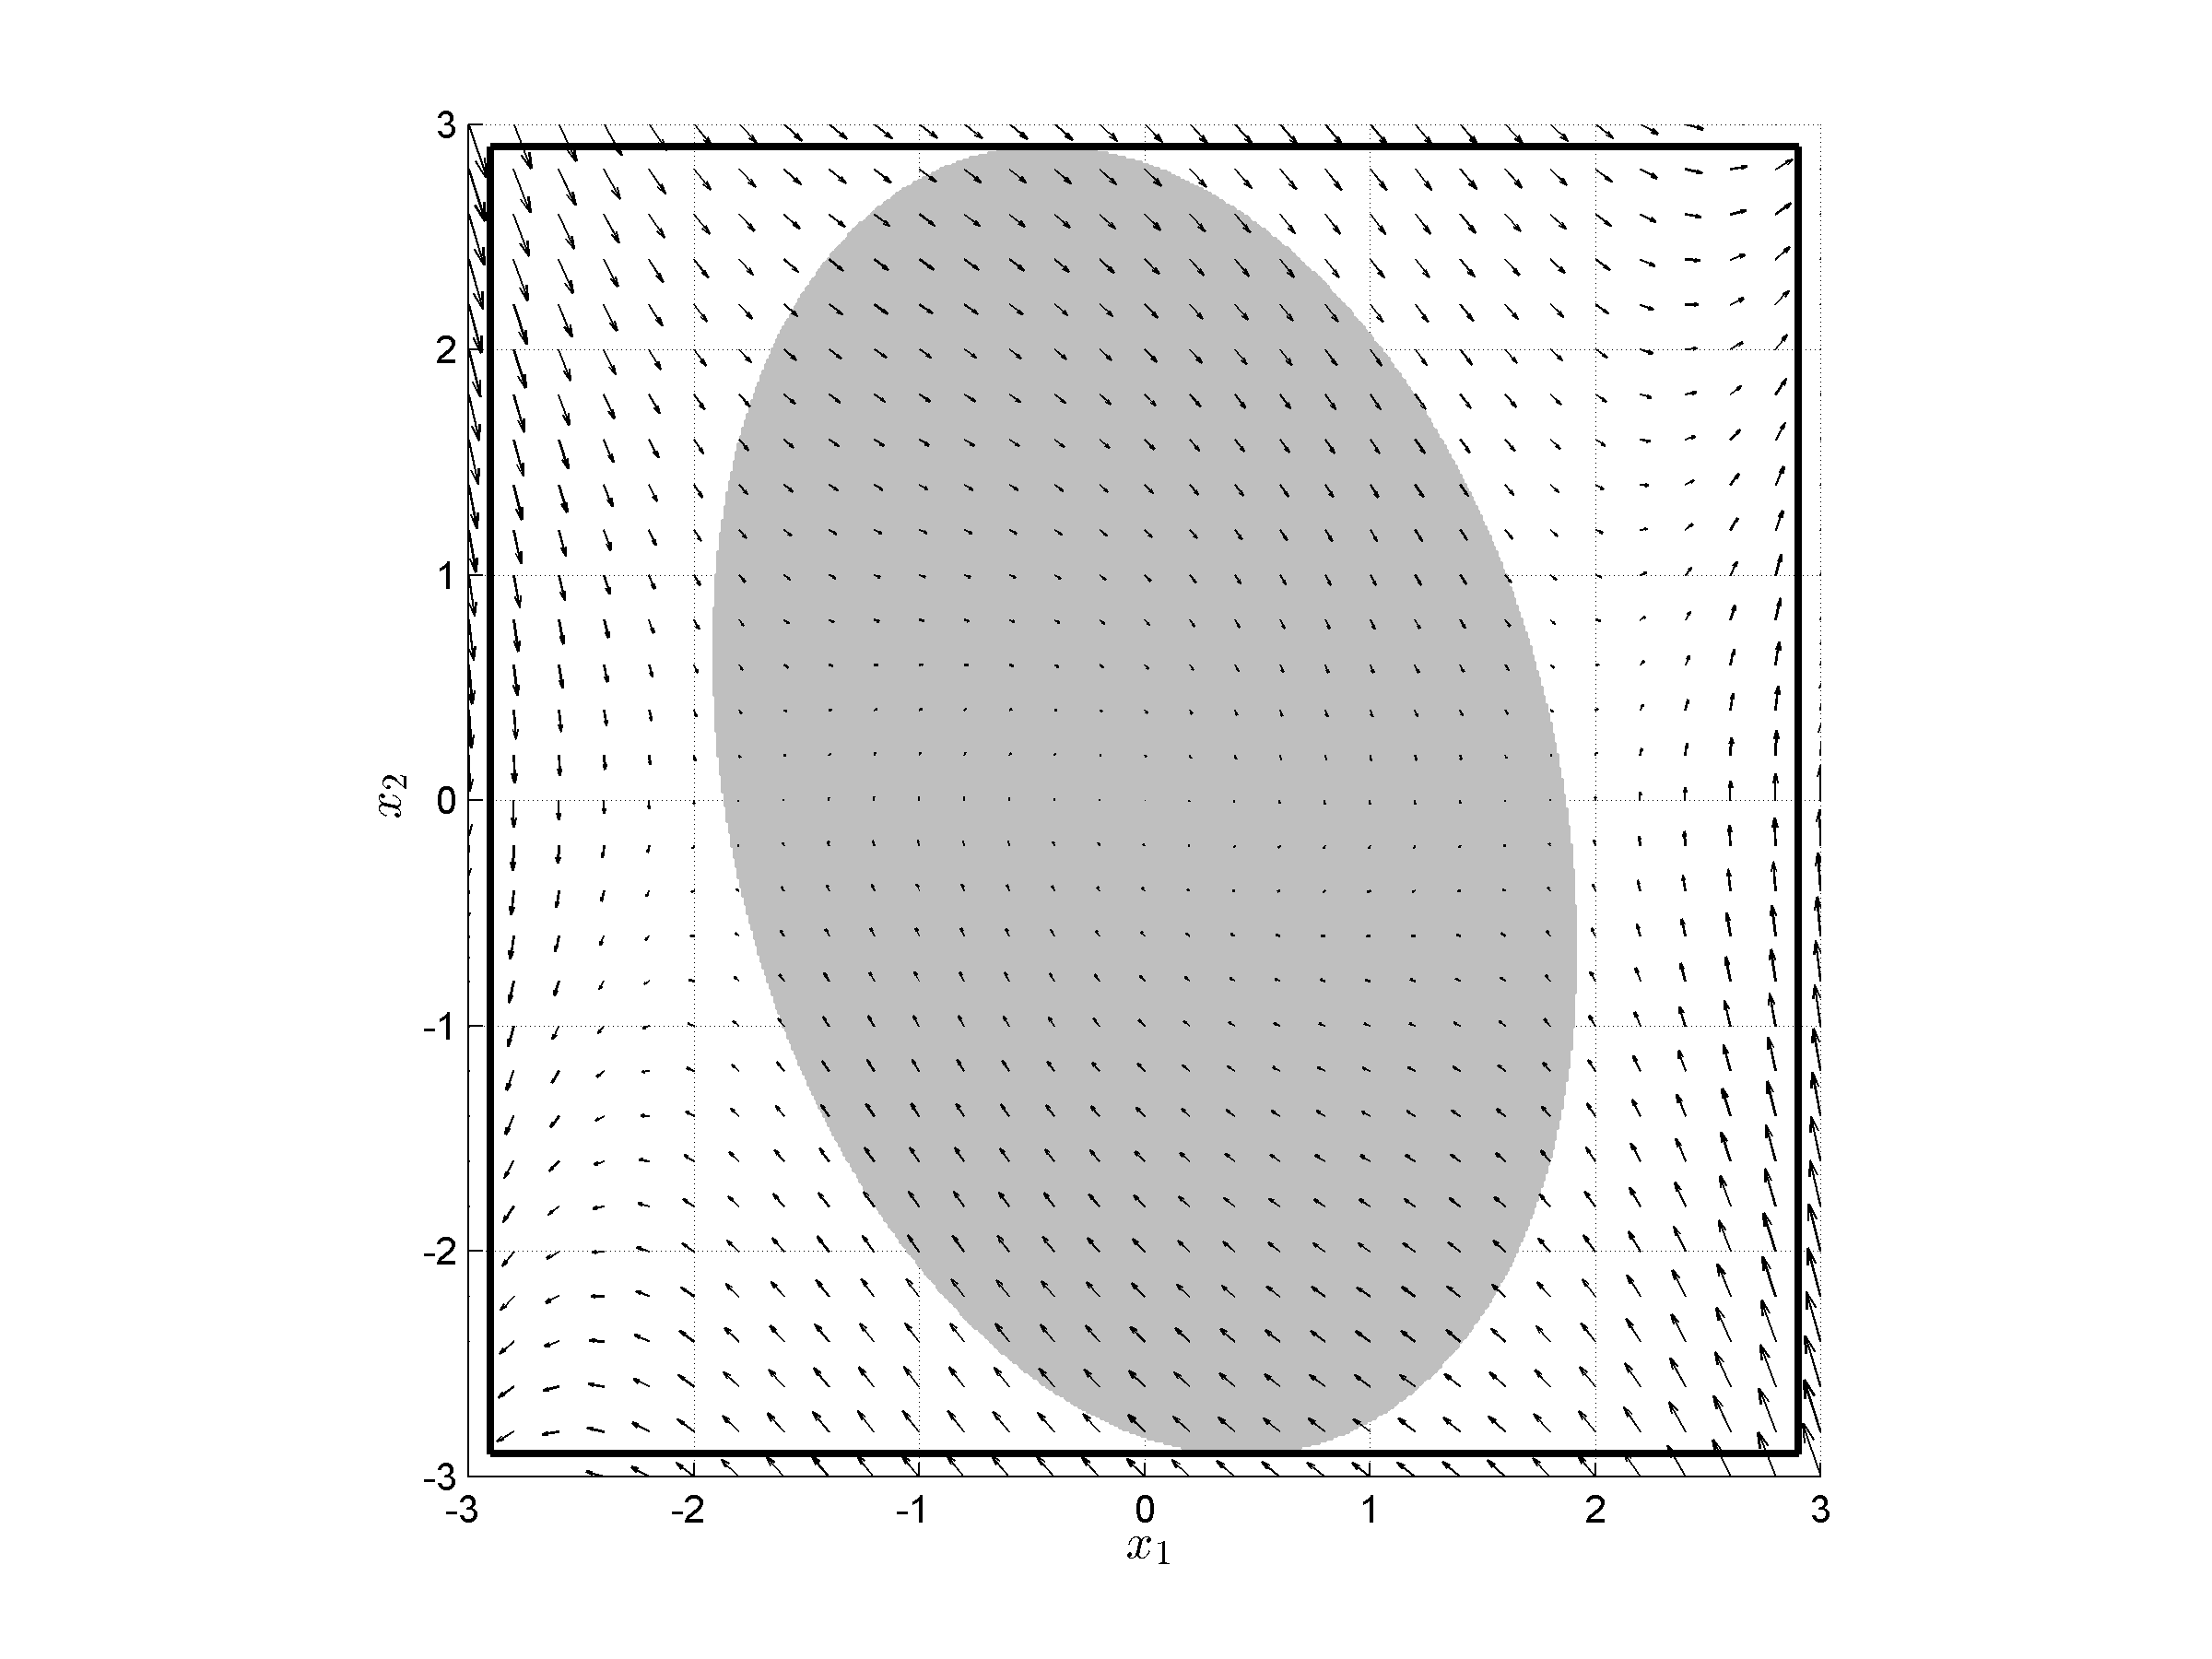
\includegraphics[height=0.7\textheight]{exemplo1_quadrado_28.eps}
  \begin{equation}
    a = \num{2.9}
  \end{equation}
\end{frame}

\againframe<2>{frame:example2}

\begin{frame}\frametitle{Exemplos}\framesubtitle{Exemplo 2 - Politopo Losangular}
  \centering
  \animategraphics[loop,controls,width=0.85\linewidth]{6}{exemplo2_}{0}{13}
\end{frame}

\begin{frame}\frametitle{Exemplos}\framesubtitle{Exemplo 2 - Politopo Quadrado}
  \centering
  \animategraphics[loop,controls,width=0.85\linewidth]{6}{exemplo2_quadrado_}{0}{8}
\end{frame}

\begin{frame}\frametitle{Exemplos}\framesubtitle{Exemplo 2 - Politopo Losangular}
  \centering
  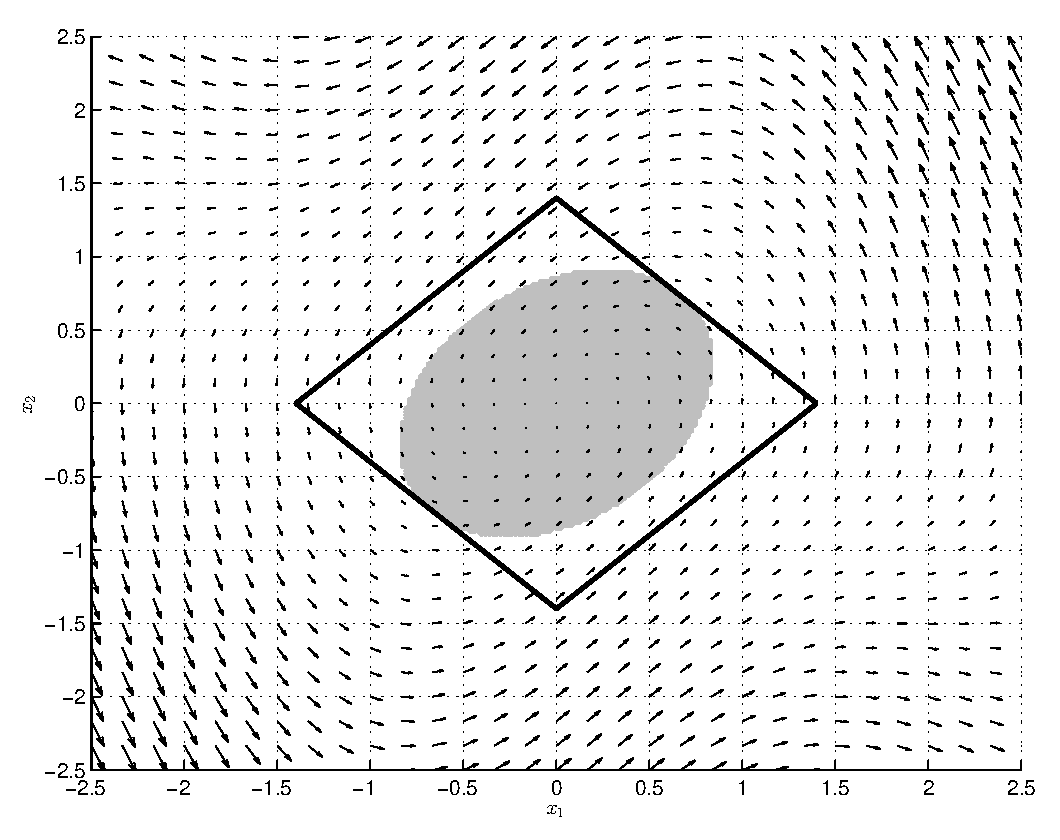
\includegraphics[height=0.7\textheight]{exemplo2_13.eps}
  \begin{equation}
    a = \num{1.4}
  \end{equation}
\end{frame}

\begin{frame}\frametitle{Exemplos}\framesubtitle{Exemplo 2 - Politopo Quadrado}
  \centering
  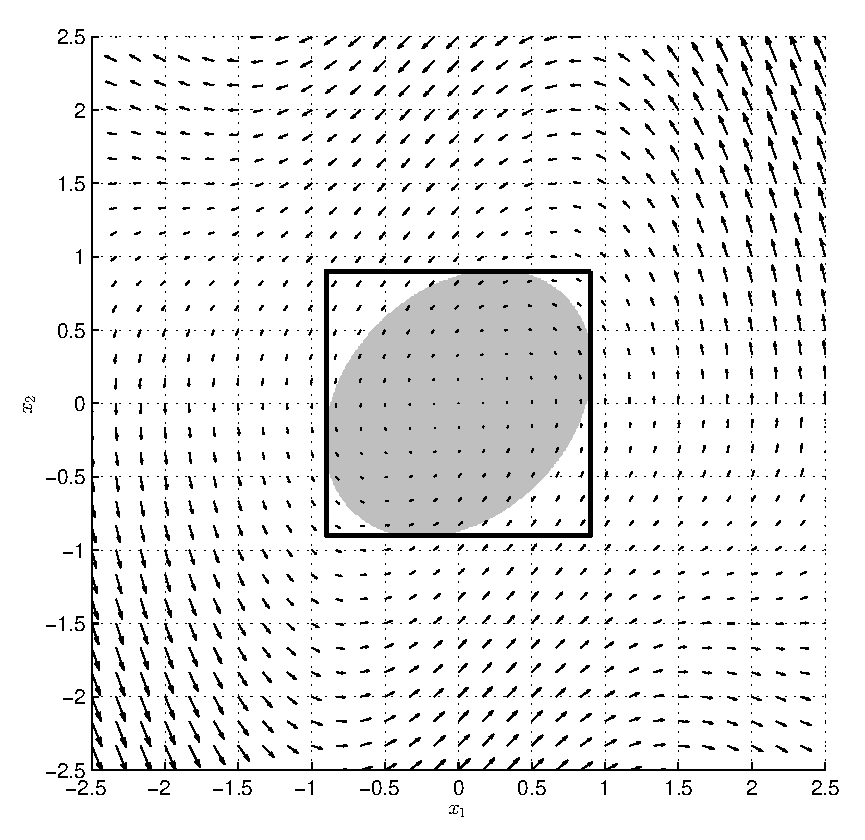
\includegraphics[height=0.7\textheight]{exemplo2_quadrado_8.eps}
  \begin{equation}
    a = \num{0.9}
  \end{equation}
\end{frame}

{
  \setbeamertemplate{navigation symbols}{}
  \againframe[noframenumbering]{frame:title}
}

\end{document}